% -*-latex-*-

\chapter{Inclusive Electron Scattering}
\label{C2}

Electron scattering is a well-proven technique to probe the internal structure of the nucleon. The electromagnetic interactions of leptons is well understood and described by Quantum Electrodynamics (QED). Distinguished by whether or not the final hadronic system is detected, the electron scattering experiments can be divided into three types: inclusive scattering, semi-inclusive and exclusive scattering. The process of inclusive electron-nucleon scattering, where only the scattered electron is detected, is discussed in this chapter. The relevant kinematic variables, the differential cross-sections and the formulation of inclusive electron scattering are presented.

\section{Kinematic Variables}
\label{C2S1}

The simplest picture of inclusive electron-nucleon scattering is with the one photon exchange approximation, which is shown in \Cref{C2S1F1}. In this scenario, an electron with four momentum $k_\mu=(E,\vec{k})$ interacts with a hadronic target. In the laboratory frame, the four momentum of the target nucleon is defined as $P_\mu=(M,\vec{0})$. For inclusive scattering, the final hadronic system is not detected, while the scattered electron is detected with the four momentum $k'_\mu=(E',\vec{k'})$. The angle between $\vec{k}$ and $\vec{k'}$ is the scattering angle $\theta$. The virtual photon exchanged by the electron and the nucleon carries a four-momentum $q_\mu=(k-k')_\mu=(\nu,\vec{q})$. Since the virtual photon is off its mass shell, $q_\mu$ satisfies $q^2\ne 0$.

\begin{figure}[tb!]
  \centering
  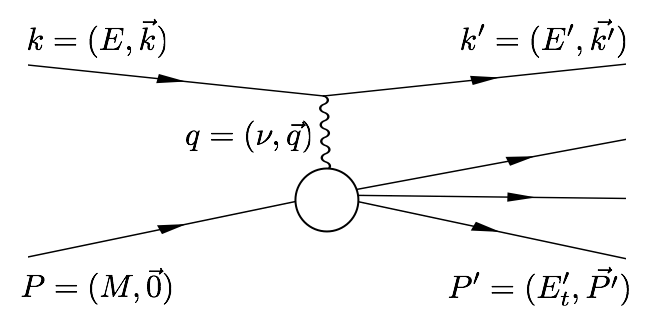
\includegraphics[width=0.6\textwidth]{figs/inclusive-scattering.png}
  \caption[Diagram for inclusive electron scattering.]{Diagram for inclusive electron scattering. \label{C2S1F1}}
\end{figure}

Two independent Lorentz invariants can be constructed from these kinematic variables. The energy transfer $\nu=(P\cdot q)/M$ and the squared four-momentum transfer $q^2=(k-k')^2$ are chosen to describe the inclusive scattering process \cite{Halzen1984}. For a space-like virtual photon, $q^2<0$, the variable $Q^2=-q^2$ is used instead of $q^2$. Since the $E$ and $E'$ are always much larger than the electron mass $m_e$ in the scattering experiments, the electron mass can be neglected. In this case, $\nu$ and $Q^2$ can be expressed as:
\begin{gather} \label{C2S1E1}
\nu = E-E', \\ \label{C2S1E2}
Q^2 = 4EE'\sin\frac{\theta}{2}.
\end{gather}
We also refer to the invariant mass of the final hadronic state:
\begin{equation} \label{C2S1E3}
W^2 = (P+q)^2 = M^2+2M\nu-Q^2.
\end{equation}
For convenience, two dimensionless scalar invariants are commonly used to replace $\nu$ and $Q^2$: the Bjorken scaling variable,
\begin{equation}  \label{C2S1E4}
x = \frac{Q^2}{2P\cdot q}=\frac{Q^2}{2M\nu},
\end{equation}
and the fraction of the electron energy loss,
\begin{equation} \label{C2S1E5}
y = \frac{P\cdot q}{P\cdot k}=\frac{E-E'}{E}.
\end{equation}

\section{Cross-Sections and Structure Functions}
\label{C2S2}

Consider the inclusive scattering of polarized electrons off polarized nucleons. The differential cross-section for detecting the final electron in the solid angle $\dd{\Omega}$ and in the final energy range ($E'$, $E'+\dd{E}$) in the laboratory frame can be written as \cite{Leader1996}:
\begin{equation} \label{C2S2E1}
\frac{\dd[2]{\sigma}}{\dd{\Omega}\dd{E'}} = \frac{\alpha^2}{Q^4}\frac{E'}{E}L_{\mu\nu}W^{\mu\nu},
\end{equation}
where $\alpha$ is the electromagnetic fine structure constant, $L_{\mu\nu}$ and $W^{\mu\nu}$ are the leptonic and hadronic tensor respectively. Defining the spin four-vector of the initial and final electron as $s_\mu$ and $s'_\mu$ respectively, the leptonic tensor $L_{\mu\nu}$ is calculable from QED:
\begin{equation} \label{C2S2E2}
L_{\mu\nu}(k,s;k's') = \sum_{s'}\bar{u}(k,s)\gamma_\mu u(k',s')\bar{u}(k',s')\gamma_\nu u(k,s),
\end{equation}
where $u$ is the Dirac spinor and $s_\mu=\bar{u}\gamma_\mu\gamma_5 u$. $L_{\mu\nu}$ can be split into symmetric (S) and antisymmetric (A) parts under $\mu$, $\nu$ interchange:
\begin{equation} \label{C2S2E3}
L_{\mu\nu}(k,s;k') = 2[L_{\mu\nu}^{(S)}(k;k') + iL_{\mu\nu}^{(A)}(k,s;k')],
\end{equation}
with
\begin{align} \label{C2S2E4}
& L_{\mu\nu}^{(S)}(k;k') = k_\mu k'_\nu+k'_\mu k_\nu-g_{\mu\nu}(k\cdot k'-m_e^2), \\ \label{C2S2E5}
& L_{\mu\nu}^{(A)}(k,s;k') = m_e\varepsilon_{\mu\nu\alpha\beta}s^\alpha q^\beta.
\end{align}
The convention for the Levi-Civita tensor is $\varepsilon_{0123}=+1$.

Due to the lack of knowledge of the hadronic vertex in \Cref{C2S1F1}, the hadronic tensor $W_{\mu\nu}$ is not yet calculable from first principles. Considering all possible transitions of the nucleon from the ground state $\ket{N(P)}$ to any excited state $\ket{X(P')}$, the hadronic tensor becomes \cite{Thomas2001}:
\begin{equation} \label{C2S2E6}
\begin{split}
W_{\mu\nu}(q;P,S) = \quad & \frac{1}{2M}\sum_X\mel{N_S(P)}{J_\mu(0)}{X(P')}\mel{X(P')}{J_\nu(0)}{N_S(P)} \\
& \cdot(2\pi)^3\delta^4(q+P-P'),
\end{split}
\end{equation}
where $S^\mu=\bar{u}(P)\gamma^\mu\gamma_5u(P)/2M$ is the hadron spin four-vector and $J_\mu$ is the electromagnetic current operator of the nucleon. Using the completeness relations of states $\ket{X}$, the tensor $W_{\mu\nu}$ can be expressed as:
\begin{equation} \label{C2S2E7}
W_{\mu\nu}(q;P,S) = \frac{1}{4\pi M}\int\dd[4]{\xi}e^{iq\cdot\xi}\mel{N_S(P)}{J_\mu(\xi)J_\nu(0)}{N_S(P)},
\end{equation}
where $\xi$ is the spatial four-vector.

As in \cref{C2S2E3}, the hadronic tensor can also be split into symmetric and antisymmetric parts:
\begin{equation} \label{C2S2E8}
W_{\mu\nu}(q;P,S) = W_{\mu\nu}^{(S)}(q;P) + iW_{\mu\nu}^{(A)}(q;P,S).
\end{equation}
Taking into account the gauge invariance and parity conservation of the electromagnetic interaction, the most general expressions of these terms are \cite{Anselmino1995}:
\begin{equation} \label{C2S2E9}
\begin{split}
W_{\mu\nu}^{(S)}(q;P) = \quad & W_1(\nu,Q^2)\left(\frac{q_\mu q_\nu}{q^2}-g_{\mu\nu}\right) \\
+ & \frac{W_2(\nu,Q^2)}{M^2}(P_\mu-\frac{P\cdot q}{q^2}q_\mu)(P_\nu-\frac{P\cdot q}{q^2}q_\nu),
\end{split}
\end{equation}
and
\begin{equation} \label{C2S2E10}
W_{\mu\nu}^{(A)}(q;P,S) = \varepsilon_{\mu\nu\alpha\beta}q^\alpha\left[G_1(\nu,Q^2)S^\beta+\frac{G_2(\nu,Q^2)}{M^2}(S^\beta P\cdot q-P^\beta S\cdot q)\right],
\end{equation}
where $W_{1,2}(\nu,Q^2)$ and $G_{1,2}(\nu,Q^2)$ are four response functions which describe the internal structure of the nucleon.

From \cref{C2S2E1,C2S2E3,C2S2E8}, one has:
\begin{equation} \label{C2S2E11}
\frac{\dd[2]{\sigma}}{\dd{\Omega}\dd{E'}}(k,s,P,S;k')= \frac{\alpha^2}{Q^4}\frac{E'}{E}\left[2L_{\mu\nu}^{(S)}W^{\mu\nu}_{(S)}-2L_{\mu\nu}^{(A)}W^{\mu\nu}_{(A)}\right].
\end{equation}
The two terms in the brackets can be separately studied by considering different polarizations of the initial electron and the target nucleon. For example, the first term is the usual unpolarized cross-section:
\begin{equation} \label{C2S2E12}
\frac{\dd[2]{\sigma}^{\mathrm{unp}}}{\dd{\Omega}\dd{E'}}(k,P;k') = \frac{1}{4}\sum_{s,S}\frac{\dd[2]{\sigma}}{\dd{\Omega}\dd{E'}}(k,s,P,S;k') = \frac{\alpha^2}{Q^4}\frac{E'}{E}2L_{\mu\nu}^{(S)}W^{\mu\nu}_{(S)}.
\end{equation}
In the polarized case, the difference of cross-sections with opposite target spins are given by the second term in \cref{C2S2E11}:
\begin{equation} \label{C2S2E13}
\frac{\dd[2]{\sigma}}{\dd{\Omega}\dd{E'}}(k,s,P,-S;k')-\frac{\dd[2]{\sigma}}{\dd{\Omega}\dd{E'}}(k,s,P,S;k') = \frac{\alpha^2}{Q^4}\frac{E'}{E}4L_{\mu\nu}^{(A)}W^{\mu\nu}_{(A)}.
\end{equation}

In practice, the response functions $W_{1,2}(\nu,Q^2)$ and $G_{1,2}(\nu,Q^2)$ are often replaced by four dimensionless structure functions in terms of the Bjorken variable $x$ and the squared four-momentum transfer $Q^2$:
\begin{align} \label{C2S2E14}
F_1(x,Q^2) & = MW_1(\nu,Q^2), \\  \label{C2S2E15}
F_2(x,Q^2) & = \nu W_2(\nu,Q^2), \\  \label{C2S2E16}
g_1(x,Q^2) & = M \nu G_1(\nu,Q^2), \\  \label{C2S2E17}
g_2(x,Q^2) & = \nu^2G_2(\nu,Q^2).
\end{align}
In terms of $F_{1,2}$ and  $g_{1,2}$, \cref{C2S2E9,C2S2E10} becomes
\begin{align}
W_{\mu\nu}^{(S)}(q;P) & = \frac{1}{M}\left(\frac{q_\mu q_\nu}{q^2}-g_{\mu\nu}\right)F_1(x,Q^2) \notag \\ \label{C2S2E18}
& \quad +\frac{1}{\nu M^2}(P_\mu-\frac{P\cdot q}{q^2}q_\mu)(P_\nu-\frac{P\cdot q}{q^2}q_\nu)F_2(x,Q^2), \\ \label{C2S2E19}
W_{\mu\nu}^{(A)}(q;P,S) & = \frac{1}{M\nu}\varepsilon_{\mu\nu\alpha\beta}q^\alpha\left[S^\beta g_1(x,Q^2)+(S^\beta-\frac{S\cdot q}{P\cdot q}P^\beta)g_2(x,Q^2)\right].
\end{align}

Using \cref{C2S2E12,C2S2E4,C2S2E18}, the differential cross-section for the inelastic scattering of unpolarized electron on unpolarized nucleon can be written as:
\begin{equation} \label{C2S2E20}
\frac{\dd[2]{\sigma}}{\dd{\Omega}\dd{E'}} = \sigma_{\mathrm{Mott}}\left[\frac{2}{M}F_1(x,Q^2)\tan^2\frac{\theta}{2}+\frac{1}{\nu}F_2(x,Q^2)\right],
\end{equation}
where $\sigma_{\mathrm{Mott}}$ is the cross-section for an electron scattered by a point-like heavy target, which can be expressed as:
\begin{equation} \label{C2S2E21}
\sigma_{\mathrm{Mott}} = \frac{\alpha^2\cos[2](\theta/2)}{4E^2\sin[4](\theta/2)}.
\end{equation}

For polarized electrons and target, the difference of cross-sections for scattering a polarized electron with spin $s$ on a polarized target with spin $S$ and that with spin $-S$ can be written using \cref{C2S2E13,C2S2E5,C2S2E19}:
\begin{equation} \label{C2S2E22}
\begin{split}
\frac{\dd[2]{\sigma}^{s,S}}{\dd{\Omega}\dd{E'}}-\frac{\dd[2]{\sigma}^{s,-S}}{\dd{\Omega}\dd{E'}} & = \frac{8m\alpha^2}{q^4}\frac{E'}{E}\frac{1}{M\nu}\Big\{[(q\cdot S)(q\cdot s)+Q^2(s\cdot S)]g_1(x,Q^2) \\
& \quad +\frac{Q^2}{M\nu}[(s\cdot S)(P\cdot q)-(q\cdot S)(P\cdot s)]g_2(x,Q^2)\Big\}.
\end{split}
\end{equation}

Considering the case that the electron is longitudinal polarized, while the nucleon are polarized along ($S$) or opposite ($-S$) to an arbitrary direction $\vec{S}$, the cross-section difference can be expressed in terms of $g_1$ and $g_2$ as:
\begin{equation} \label{C2S2E23}
\begin{split}
& \frac{\dd[2]{\sigma}^{\rightarrow,S}}{\dd{\Omega}\dd{E'}}-\frac{\dd[2]{\sigma}^{\rightarrow,-S}}{\dd{\Omega}\dd{E'}} = -\frac{4\alpha^2}{Q^2}\frac{E'}{E} \\
& \quad \times\frac{1}{\nu M}\left[(E\cos\alpha+E'\cos\Theta)g_1(x,Q^2)+\frac{2EE'}{\nu}(\cos\Theta-\cos\alpha)g_2(x,Q^2)\right],
\end{split}
\end{equation}
where $\alpha$ is the angle between the incident electron momentum $\vec{k}$ and the direction of the target polarization $\vec{S}$. $\Theta$ is the angle between the outgoing electron momentum $\vec{k'}$ and $\vec{S}$. If $\phi$ is the azimuthal angle between the scattering plane ($\vec{k}$, $\vec{k'}$) and the polarization plane ($\vec{k}$, $\vec{S}$), $\cos\Theta$ can be expressed as:
\begin{equation} \label{C2S2E24}
\cos\Theta = \sin\theta\sin\alpha\cos\phi+\cos\theta\cos\alpha,
\end{equation}
where $\theta$ is the scattering angle. See \Cref{C2S2F1} for the definitions of the angles $\alpha$, $\theta$ and $\phi$.

\begin{figure}[tb!]
  \centering
  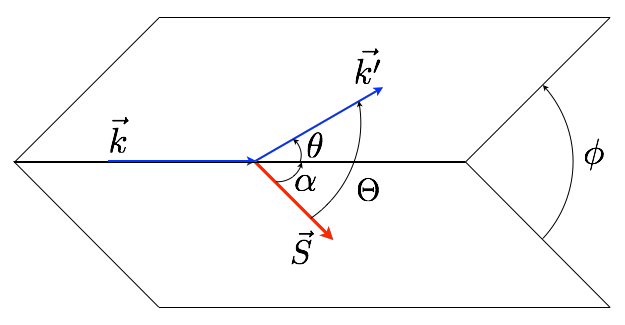
\includegraphics[width=0.5\textwidth]{figs/angles-of-polarized-scattering.png}
  \caption[Angular relations of polarized electron scattering.]{Angular relations of polarized electron scattering. \label{C2S2F1}}
\end{figure}

Therefore, one can derive the cross-section difference for some special values of $\alpha$. For the case that the target nucleons are longitudinally polarized, $\alpha=0$ and $\Theta=\theta$, the cross-section difference for the electron scattering on the nucleon polarized parallel ($\buildrel\rightarrow\over\Rightarrow$) or anti-parallel ($\buildrel\rightarrow\over\Leftarrow$) to the initial electron direction (i.e. the electron spin direction since the electron is longitudinal polarized) can be expressed as:
\begin{equation} \label{C2S2E25}
\frac{\dd[2]{\sigma}^{\buildrel\rightarrow\over\Leftarrow}}{\dd{\Omega}\dd{E'}}-\frac{\dd[2]{\sigma}^{\buildrel\rightarrow\over\Rightarrow}}{\dd{\Omega}\dd{E'}}=\frac{4\alpha^2E'}{\nu MQ^2E}\left[(E+E'\cos\theta)g_1(x,Q^2)-2Mxg_2(x,Q^2)\right].
\end{equation}
If the target nucleons are transversely polarized and the nucleon spin lies in the scattering plane, $\alpha=\pi/2$ and $\phi=0$ or $\pi$, the cross-section difference can be expressed as:
\begin{equation} \label{C2S2E26}
\frac{\dd[2]{\sigma}^{\rightarrow\Uparrow}}{\dd{\Omega}\dd{E'}}-\frac{\dd[2]{\sigma}^{\rightarrow\Downarrow}}{\dd{\Omega}\dd{E'}}=\frac{4\alpha^2E'^2}{\nu MQ^2E}\sin\theta\left[g_1(x,Q^2)+\frac{2E}{\nu}g_2(x,Q^2)\right].
\end{equation}

\section{Structure Functions in the Parton Model}
\label{C2S3}

In the last Section, the hadronic tensor $W_{\mu\nu}$ was written in term of the structure functions $F_{1,2}$ and $g_{1,2}$. One of the important feature of the structure functions is their scaling behavior in the Bjorken limit \cite{Bjorken1969}:
\begin{equation} \label{C2S3E1}
Q^2\to\infty, \text{ and } \nu\to\infty, \text{ with } x=\frac{Q^2}{2M\nu} \text{ fixed}.
\end{equation}
It turns out that to a very good approximation the structure functions are independent of $Q^2$ and can be written as $F_{1,2}(x)$ and $g_{1,2}(x)$. This phenomenon known as Bjorken scaling was first discovered at the Stanford Linear Accelerator \cite{Kendall1991}.

The parton model of Feynman \cite{Feynman1969} provides a clear explanation for the Bjorken scaling. Any object with a finite size must have a form factor which introduces some $Q^2$ dependence. Thus, the fact of Bjorken scaling implies that the nucleon must contain point-like constituents, which are named partons. Since the structure functions are Lorentz invariant, the parton model can be formulated in any frame. For convenience, the infinite momentum frame, where the nucleon is moving with momentum approaching $\infty$ along the $z$-direction, is chosen to formulate the parton model. Due to time dilatation, there is no time for interaction between the partons in this frame and the process can be viewed as the incoherent sum of elastic scattering from non-interacting partons, that is: the hadronic tensor $W_{\mu\nu}$ is given in terms of the elementary quark tensor $w_{\mu\nu}$ by \cite{Leader1996}:
\begin{equation} \label{C2S3E2}
W_{\mu\nu}(q;P,S) = \sum_{i,s}e_i^2\frac{1}{2P\cdot q}\int_0^1\frac{\dd{x'}}{x'}\delta(x'-x)n_i(x',s;S)w_{\mu\nu}(x',q,s),
\end{equation}
where the $\sum_i$ runs over quarks and antiquarks, and $n_i$ is the number density of the quark $i$ with charge $e_i$. Since quarks are point-like particles in the model, the quark tensor $w_{\mu\nu}$ is similar to the lepton tensor $L_{\mu\nu}$.

To evaluate the structure functions from \cref{C2S3E2}, four projection operators are defined as \cite{Anselmino1995}:
\begin{align} \label{C2S3E3}
P_1^{\alpha\beta} & \equiv \frac{1}{4}\left[\frac{1}{a}P^\alpha P^\beta-g^{\alpha\beta}\right], \\ \label{C2S3E4}
P_2^{\alpha\beta} & \equiv \frac{3P\cdot q}{4a}\left[\frac{1}{a}P^\alpha P^\beta-\frac{1}{3}g^{\alpha\beta}\right],
\end{align}
where $a=(P\cdot q)/2x+M^2$, and
\begin{align} \label{C2S3E5}
P_3^{\alpha\beta} & \equiv \frac{(P\cdot q)^2}{bM^2(q\cdot S)}\left[(q\cdot S)S_\lambda+q_\lambda\right]P_\eta\varepsilon^{\alpha\beta\lambda\eta}, \\ \label{C2S3E6}
P_4^{\alpha\beta} & \equiv \frac{1}{b}\left\{\left[\frac{(P\cdot q)^2}{M^2}+2(P\cdot q)x\right]S_\lambda+(q\cdot S)q_\lambda\right\}P_\eta\varepsilon^{\alpha\beta\lambda\eta},
\end{align}
where
\begin{equation} \label{C2S3E7}
b = -4M\left[\frac{(P\cdot q)^2}{M^2}+2(P\cdot q)x-(q\cdot S)^2\right].
\end{equation}
With these projectors, one has:
\begin{equation} \label{C2S3E8}
\begin{aligned}
P_1^{\alpha\beta}W_{\alpha\beta} & = F_1, & \qquad P_2^{\alpha\beta}W_{\alpha\beta} & = F_2, \\
P_3^{\alpha\beta}W_{\alpha\beta} & = g_1, & \qquad P_4^{\alpha\beta}W_{\alpha\beta} & = g_1+g_2.
\end{aligned}
\end{equation}

Applying the projection operator \cref{C2S3E3,C2S3E4,C2S3E5,C2S3E6} to \cref{C2S3E2}, one can obtain the relations between the nucleon structure functions and the parton distribution functions:
\begin{align} \label{C2S3E9}
F_1(x) & = \frac{1}{2}\sum_ie_i^2q_i(x), \\ \label{C2S3E10}
F_2(x) & = x\sum_ie_i^2q_i(x) = 2xF_1(x), \\ \label{C2S3E11}
g_1(x) & = \frac{1}{2}\sum_ie_i^2\Delta q_i(x),
\end{align}
where $q(x)=q^\uparrow(x)+q^\downarrow(x)$ is the unpolarized parton distribution function, which is the probability of finding a quark carrying the fraction $x$ of the momentum of the nucleon. $\Delta q(x)=q^\uparrow(x)-q^\downarrow(x)$ is the polarized parton distribution function, where $q^\uparrow(x)$ ($q^\downarrow(x)$) is the number density of the quark carrying the fraction $x$ of the momentum of the nucleon when it is aligned parallel (or anti-parallel) to the nucleon spin direction. \cref{C2S3E10} is a relation between $F_1$ and $F_2$ which is also known as the Callan-Gross relation \cite{Callan1969}.

The transverse polarized structure function $g_2(x)$ is zero in the naive parton model described above. However, if one allows the constituent quarks to have an intrinsic transverse momentum in the nucleon, the value of $g_2$ can be non-zero.
The interpretation of $g_2(x)$ in the naive parton model is not as simple as the other structure functions \cite{Thomas2001}. It carries the information of the quark-gluon interaction inside the nucleon, which will be introduced in the next chapter.

The scaling behavior of the structure functions is only valid at the Bjorken limit as mentioned at the beginning of this section. At finite $Q^2$, the Bjorken scaling is only a good approximation since the interaction between quarks can not be ignored. QCD radiative corrections need to be included in the cross-section calculation. \Cref{C2S3F1} shows two basic processes which cannot be separated from the major process of electron scattering. In particular, the electron scattering process from a quark cannot be separated from the scattering processes with a soft gluon radiated. As the radiative effects in QED, the soft gluon radiation also gives rise to an infinite cross-section which can be renormalized if all other processes at the same order are included.

\begin{figure}[tb!]
  \centering
  \begin{subfigure}[t]{0.35\textwidth}
    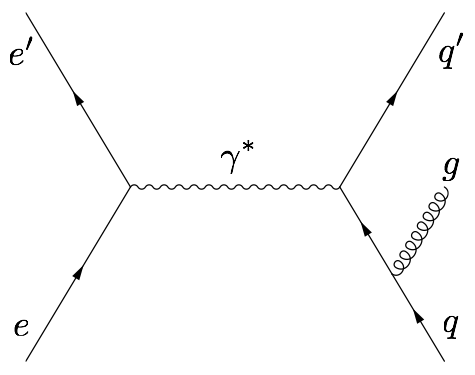
\includegraphics[width=\textwidth]{figs/gluon-radiation-a.png}
  \end{subfigure}
  \begin{subfigure}[t]{0.35\textwidth}
    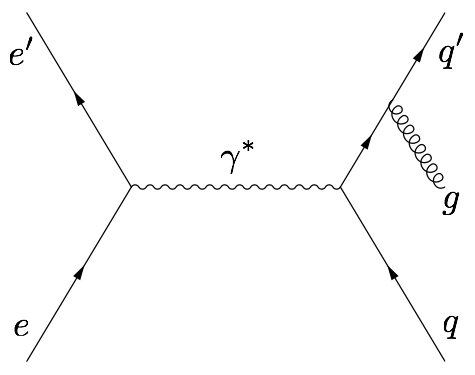
\includegraphics[width=\textwidth]{figs/gluon-radiation-b.png}
  \end{subfigure}
  \caption[Gluon radiation in electron-quark scattering.]{Radiating process which cannot be separated from the basic process of electron scattering. \label{C2S3F1}}
\end{figure}

\begin{figure}[p!]
  \centering
  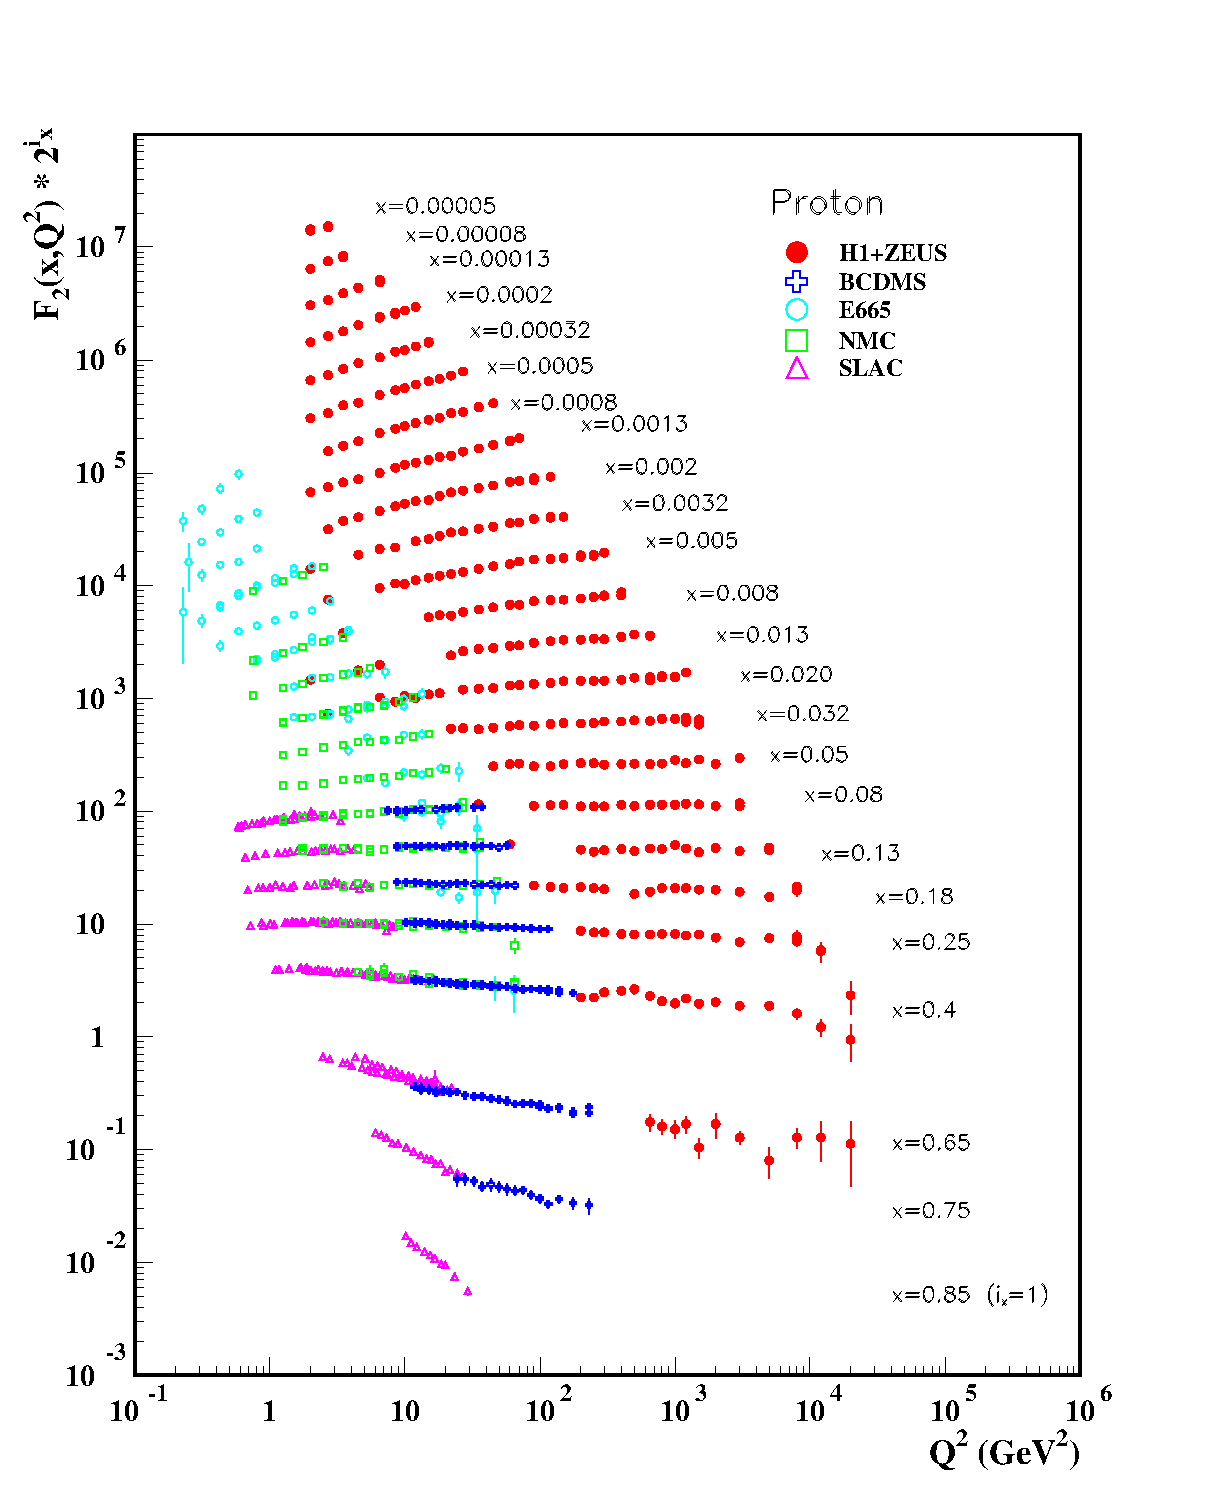
\includegraphics[width=\textwidth,trim=0 0 10mm 25mm]{figs/f2collider-logf2}
  \caption[The $Q^2$ dependence of the proton structure function $F_2^p$.]{The proton structure function $F_2^p$ measured in electromagnetic scattering of electrons and positrons off protons (collider experiments H1 and ZEUS for $Q^2\geq 2\text{ GeV}^2$) and for electrons (SLAC) and muons (BCDMS, E665, NMC) on a fixed target. The data are plotted as a function of $Q^2$ in bins of fixed $x$. For the purpose of plotting, $F_2^p$ has been multiplied by $2^{i_x}$, where $i_x$ is the number of the $x$ bin, ranging from $i_x= 1$ ($x=0.85$) to $i_x=24$ ($x=0.00005$). Plot reproduced from \cite{Olive2014}. \label{C2S3F2}}
\end{figure}

This variation of the structure functions with $Q^2$ is referred to as QCD evolution. After renormalization, the gluon radiative correction gives a logarithmic dependence to the cross-section. \Cref{C2S3F2} shows the experimental $Q^2$-dependence of the proton $F_2$ structure function for a large range of $x$ \cite{Olive2014}. By incorporating the $Q^2$-dependence into the definition of the parton distributions, the expression of structure functions can be generalized as:
\begin{align} \label{C2S3E12}
F_1(x,Q^2) & = \frac{1}{2}\sum_ie_i^2q_i(x,Q^2), \\ \label{C2S3E13}
g_1(x,Q^2) & = \frac{1}{2}\sum_ie_i^2\Delta q_i(x,Q^2).
\end{align}
Now $q(x,Q^2)\dd{x}$ should be interpreted as the probability of finding a quark in the nucleon with momentum fraction between $x$ and $x+\dd{x}$ when viewed with a resolution determined by $Q^2$. If one probes the proton at low $Q^2$, the wavelength is large ($1/\sqrt{Q^2}$) and the spatial resolution is poor. The structure functions is expected to be dominated by the valence quarks at this case. As $Q^2$ increases, more and more $q\bar{q}$ pairs and gluons can be seen since the resolution becomes better.

The QCD evolution can be calculated from perturbative QCD in the leading order. The Altarelli Parisi, or DGLAP equations developed by Gribov and Lipatov \cite{Gribov1972}, Dokshitzer \cite{Dokshitzer1977} and Altarelli and Parisi \cite{Altarelli1977} provide a method to calculate the $Q^2$-dependence of the structure functions. These equations are first-order integro-differential equations. Thus, the parton distributions can be calculated at any $Q^2$ scale where perturbative QCD applies if the distributions at some particular scale is known.

\section{Virtual Photon-absorption Cross-Sections: An Alternative Formulation}
\label{C2S4}

The previous sections revealed that the inclusive scattering process can be formulated with four structure functions. Before we go further, it is worth introducing an equivalent formulation of the inclusive scattering process in which the cross-section is parameterized in terms of four virtual photon-absorption cross-sections.

\subsection{Virtual Photon-absorption Cross-Sections}
\label{C2S4SS1}

As shown in \Cref{C2S1F1}, the inclusive scattering process is equivalent to absorption of a virtual photon on a nucleon. In the center of mass (c.m.) frame of the hadronic intermediate state, the four-momentum of the virtual photon is given by ($\omega_\gamma$, $\vec{k}_\gamma$), which can be expressed as \cite{Drechsel2004}:
\begin{equation} \label{C2S4E1}
\omega_\gamma = \frac{M\nu-Q^2}{W}, \qquad \vec{k}_\gamma = \frac{M}{W}\vec{q}.
\end{equation}
where $|\vec{q}|=\sqrt{\nu^2+Q^2}$ is the lab photon momentum. Since $\omega_\gamma$ vanishes at $\nu=Q^2/M$ and therefore is inconvenient in the context of the multipole expansion, one can define the ``equivalent photon energy'' or the virtual photon flux $K$ to replace $\omega_\gamma$ according to Hand's definition \cite{Hand1963}:
\begin{equation} \label{C2S4E2}
K = K_H = \nu(1-x) = \frac{W^2-M^2}{2M}.
\end{equation}
An alternative convention could be Gilman's definition \cite{Gilman1968}:
\begin{equation} \label{C2S4E3}
K = K_G = |\vec{q}| = \sqrt{\nu^2+Q^2}.
\end{equation}
\cref{C2S4E2,C2S4E3} reduce to $\nu$ for the real photon scattering at $Q^2=0$. However, at intermediate $Q^2$, the photon flux is strongly convention dependent.

The inclusive electron-nucleon scattering can then be parameterized in terms of a flux factor and four partial cross-sections \cite{Drechsel2001}:
\begin{equation} \label{C2S4E4}
\frac{\dd{\sigma}}{\dd{\Omega}\dd{E'}} = \Gamma_V[\sigma_T+\epsilon\sigma_L-hP_x\sqrt{2\epsilon(1-\epsilon)}\slt-hP_z\sqrt{1-\epsilon^2}\stt],
\end{equation}
where $h$ is the helicity of the longitudinally polarized electron and $P_z$ and $P_x$ denote the components of the target polarization parallel and perpendicular to the virtual photon momentum $\vec{q}$ in the scattering plane of the electron respectively. The $\epsilon$ is the photon polarization and $\Gamma_V$ is the virtual photon flux factor:
\begin{equation*}
\epsilon = \frac{1}{1+2(1+\nu^2/Q^2)\tan^2\theta/2}, \qquad \Gamma_V = \frac{\alpha}{2\pi^2}\frac{E'}{E}\frac{K}{Q^2}\frac{1}{1-\epsilon}.
\end{equation*}
The four partial cross-sections are the transverse ($\sigma_T$) and longitudinal ($\sigma_L$) cross-sections and two interference terms: the longitudinal-transverse cross-sections ($\slt$) and the transverse-transverse cross-sections ($\stt$). $\sigma_T$ and $\sigma_L$ represent the cross-sections for absorption of transverse and longitudinal virtual photons respectively. $\sigma_L$ vanishes in the $Q^2=0$ (real photon) limit since the real photon is transversely polarized. Therefore, the total photon-absorption cross-section is given by $\sigma_T$ in the real photon limit. The two spin-flip cross-sections can only be measured by double-polarization experiments.

The partial cross-sections $\sigma_T$ and $\stt$ can be expressed in terms of the helicity dependent photo-absorption cross-sections $\sigma_{1/2}$ and $\sigma_{3/2}$. The subscripts refer to the total spin of the photon plus the target nucleon. \Cref{C2S4F1} shows the two different situations. These helicity dependent cross-sections are related to $\sigma_T$ and $\stt$ through:
\begin{equation} \label{C2S4E5}
\sigma_T = \frac{1}{2}(\sigma_{1/2}+\sigma_{3/2}), \qquad \stt = \frac{1}{2}(\sigma_{1/2}-\sigma_{3/2}).
\end{equation}

\begin{figure}[tb!]
  \centering
  \begin{subfigure}[t]{0.4\textwidth}
    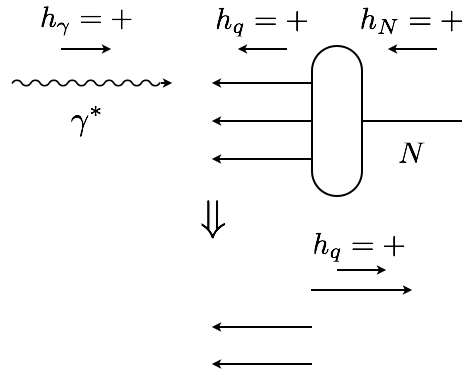
\includegraphics[width=\textwidth]{figs/photon-absorption-a.png}
    \subcaption{{}\label{C2S4F1A}}
  \end{subfigure}
  \qquad
  \qquad
  \begin{subfigure}[t]{0.4\textwidth}
    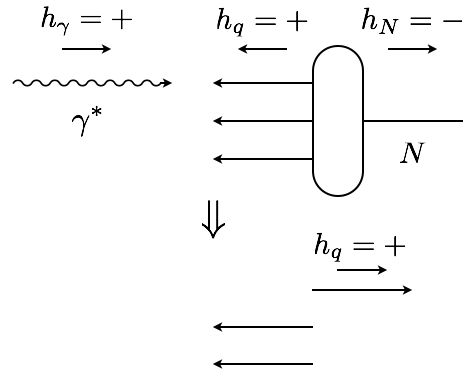
\includegraphics[width=\textwidth]{figs/photon-absorption-b.png}
    \subcaption{{}\label{C2S4F1B}}
  \end{subfigure}
  \caption[Schematic of the helicity dependent cross-sections $\sigma_{1/2}$ and $\sigma_{3/2}$.]{The helicity dependent cross-sections for a positive helicity virtual photon ($h_\gamma=+$) to be absorbed by a polarized nucleon (here $h_N=\pm$ means $h_N=\pm 1/2$): (a) $\sigma_{1/2}$ and (b) $\sigma_{3/2}$. \label{C2S4F1}}
\end{figure}

The relations between the structure functions and the photo-absorption cross-sections can be written as \cite{Thomas2001,Drechsel2003}:
\begin{align} \label{C2S4E6}
\sigma_T & = AF_1, \\ \label{C2S4E7}
\sigma_L & = A\left[\frac{(1+\gamma^2)M}{\gamma^2\nu}F_2-F_1\right], \\ \label{C2S4E8}
\stt & = A(g_1-\gamma^2g_2), \\ \label{C2S4E9}
\slt & = A\gamma(g_1+g_2),
\end{align}
where $\gamma=Q/\nu$ and $A=4\pi^2\alpha/MK$.

\subsection{Compton Scattering}
\label{C2S4SS2}

Now consider the elastic real photon scattering process $\gamma(k)+N(P)\rightarrow\gamma(k')+N(P')$. The four-momentum of the incident and scattered real photon is $k=(\nu,\vec{k})$ and $k'=(\nu',\vec{k'})$ respectively with $k^2=k'^2=0$. In the laboratory frame, the four-momentum of the nucleon is $P=(M,0)$. If we denote the scattering angle by $\theta$ in the laboratory frame, the energy and momentum conservation gives \cite{Thomas2001}:
\begin{equation} \label{C2S4E10}
\nu' = \frac{\nu}{1+\frac{\nu}{M}(1-\cos\theta)}.
\end{equation}

The polarization of the incident and scattered photons can be characterized by two linear polarization vectors $\epsilon^\mu$ and $\epsilon'^\nu$. Due to the transverse nature of real photons, we choose:
\begin{equation} \label{C2S4E11}
\begin{split}
\epsilon^\mu = (0,\vec{\epsilon}), & \quad \vec{k}\cdot\vec{\epsilon} = 0, \\
\epsilon'^\nu = (0,\vec{\epsilon'}), & \quad \vec{k'}\cdot\vec{\epsilon'} = 0.
\end{split}
\end{equation}
We can choose a coordinate system such that the $z$-axis coincides with the direction of $\vec{k}$. The polarization vector of a linearly polarized photon can be expressed as the linear combination of two unit vectors:
\begin{equation} \label{C2S4E12}
\vec{\epsilon}_x = (1,0,0), \quad \vec{\epsilon}_y = (0,1,0).
\end{equation}
The circularly polarized photons are given by:
\begin{equation} \label{C2S4E13}
\vec{\epsilon}_{\lambda=1} = \frac{1}{\sqrt{2}}(\vec{\epsilon}_x+i\vec{\epsilon}_y), \quad \vec{\epsilon}_{\lambda=-1} = \frac{1}{\sqrt{2}}(\vec{\epsilon}_x-i\vec{\epsilon}_y),
\end{equation}
with $\vec{\epsilon}^{\;\star}_{\lambda'}\cdot\vec{\epsilon}_{\lambda}=\delta_{\lambda'\lambda}$.

The differential cross-section for real Compton scattering is given by:
\begin{equation} \label{C2S4E14}
\frac{\dd{\sigma}}{\dd{\nu}} = \left(\frac{\nu'}{8\pi M\nu}\right)^2|T_{fi}|^2.
\end{equation}
Using the polarization vectors defined in \cref{C2S4E11}, the transition matrix $T_{fi}$ of real Compton scattering can be written as \cite{Thomas2001}:
\begin{equation} \label{C2S4E15}
T_{fi} = e^2\epsilon'^{\star\mu}\epsilon^\nu T_{\mu\nu}(k',P';k,P),
\end{equation}
with
\begin{equation} \label{C2S4E16}
T_{\mu\nu} = i\int\dd[4]{x}e^{ik'\cdot x}\mel{N(P')}{\mathcal{T}\{J_\mu(x)J_\nu(0)\}}{N(P)},
\end{equation}
here $\mathcal{T}$ is the time-ordering operator.

For forward scattering with $\vec{k'}=\vec{k}$, the forward Compton scattering amplitude can be expressed as \cite{Drechsel2003}:
\begin{equation} \label{C2S4E17}
T(\nu,\theta=0) = \vec{\epsilon}\,'^\star\cdot\vec{\epsilon}f(\nu)+i\vec{\sigma}\cdot(\vec{\epsilon}\,'^\star\times\vec{\epsilon}\,)g(\nu),
\end{equation}
where $\vec{\sigma}$ are the Pauli spin matrices and $f(\nu)$, $g(\nu)$ represents the spin non-flip and flip amplitudes respectively.

According to the optical theorem, the total photon absorption cross-sections is related to the imaginary part of the forward Compton scattering amplitudes by:
\begin{equation} \label{C2S4E18}
\begin{split}
\Im f(\nu) & = \frac{\nu}{8\pi}(\sigma_{1/2}(\nu)+\sigma_{3/2}(\nu)) = \frac{\nu}{4\pi}\sigma_T(\nu), \\
\Im g(\nu) & = \frac{\nu}{8\pi}(\sigma_{1/2}(\nu)-\sigma_{3/2}(\nu)) = \frac{\nu}{4\pi}\stt(\nu).
\end{split}
\end{equation}

The amplitudes $f(\nu)$ and $g(\nu)$ can be expanded in powers of $\nu$ via the low energy theorem (LET) of Low \cite{Low1954} and Gell-Mann and Goldberger \cite{Gellmann1954b}:
\begin{align} \label{C2S4E19}
f(\nu) & = -\frac{Z^2e^2}{4\pi M}+(\alpha+\beta)\nu^2+\mathcal{O}(\nu^4), \\ \label{C2S4E20}
g(\nu) & = -\frac{\kappa^2e^2}{8\pi M^2}\nu+\gamma_0\nu^3+\mathcal{O}(\nu^5),
\end{align}
where $Z$ is the charge in the unit of elementary charge, and $\kappa$ is the anomalous magnetic moment in the unit of nuclear magneton. The leading term of the spin non-flip amplitude gives the classical Thomson scattering result. The $\mathcal{O}(\nu^2)$ term contains information of the internal structure and appears as the sum of the electric and magnetic dipole polarizabilities $\alpha$ and $\beta$. The $\mathcal{O}(\nu^3)$ term of the spin flip amplitude is related to the forward spin polarizability $\gamma_0$ with information of the spin structure.

By use of the optical theorem, the Kramers-Kronig dispersion relations can be derived for $f(\nu)$ and $g(\nu)$, which gives:
\begin{align} \label{C2S4E21}
\Re f(\nu) & = f(0)+\frac{\nu^2}{2\pi^2}\pv{\int_{\nu_0}^\infty\dd{\nu'}\frac{\sigma_T(\nu')}{\nu'^2-\nu^2}}, \\ \label{C2S4E22}
\Re g(\nu) & = \frac{\nu}{4\pi^2}\pv{\int_{\nu_0}^\infty\dd{\nu'}\nu'\frac{\sigma_{1/2}(\nu')-\sigma_{3/2}(\nu')}{\nu'^2-\nu^2}},
\end{align}
where $\pv$ means the principal value of the integral. $\nu_0$ is introduced to ensure that the integral converges. Thus, the two integrals can be expand as a Taylor series in $\nu$:
\begin{align} \label{C2S4E23}
\Re f(\nu) & = f(0)+\sum_{n=1}\left(\frac{1}{2\pi^2}\int_{\nu_0}^\infty\dd{\nu'}\frac{\sigma_T(\nu')}{\nu'^{2n}}\right)\nu^{2n}, \\ \label{C2S4E24}
\Re g(\nu) & = \sum_{n=1}\left(\frac{1}{4\pi^2}\int_{\nu_0}^\infty\dd{\nu'}\frac{\sigma_{1/2}(\nu')-\sigma_{3/2}(\nu')}{\nu'^{2n-1}}\right)\nu^{2n-1}.
\end{align}

By comparing \cref{C2S4E23,C2S4E24} with \cref{C2S4E19,C2S4E20}, we can obtain Baldin's sum rule \cite{Baldin1960,Lapidus1963} from the $\mathcal{O}(\nu^2)$ term of spin non-flip amplitude $f(\nu)$:
\begin{equation} \label{C2S4E25}
\alpha+\beta = \frac{1}{2\pi^2}\int_{\nu_0}^\infty\dd{\nu'}\frac{\sigma_T(\nu')}{\nu'^{2}}.
\end{equation}
From the leading term of the spin flip amplitude $g(\nu)$, we can obtain the Gerasimov-Drell-Hearn (GDH) sum rule \cite{Gerasimov1966,Drell1966}:
\begin{equation} \label{C2S4E26}
-2\pi^2\alpha\frac{\kappa^2}{M^2} = \int_{\nu_0}^\infty\dd{\nu'}\frac{\sigma_{1/2}(\nu')-\sigma_{3/2}(\nu')}{\nu'}\equiv I,
\end{equation}
where $\alpha=e^2/4\pi$ is the fine structure constant. And we can also obtain a relation for the forward spin polarizability \cite{Gellmann1954a,Gellmann1954b}:
\begin{equation} \label{C2S4E27}
\gamma_0 = \frac{1}{4\pi^2}\int_{\nu_0}^\infty\dd{\nu'}\frac{\sigma_{1/2}(\nu')-\sigma_{3/2}(\nu')}{\nu'^3}.
\end{equation}

The above discussion could be generalized if we treat the real photon as virtual by replacing $k$ with $q$ and assume $q^2\neq 0$. This is known as the double virtual Compton scattering (VVCS). Comparing \cref{C2S4E16} with \cref{C2S2E7}, we notice that the difference between $T_{\mu\nu}$ and the hadronic tensor $W_{\mu\nu}$ is the time ordering operator $\mathcal{T}$ of the electromagnetic currents. Actually $W_{\mu\nu}$ is related to the forward virtual Compton tensor $T_{\mu\nu}$ by \cite{Thomas2001}:
\begin{equation} \label{C2S4E190}
W_{\mu\nu}(q,P) = \frac{1}{2\pi M}\Im T_{\mu\nu}(q,P;q,P).
\end{equation}
This relation implies that the components of the hadronic tensor, e.g., the structure functions, are related to the forward double VVCS amplitudes by the Kramers-Kronig dispersion relations. We will continue the discussion of these relations in \Cref{C4}.

%%%%%%%%%%%%%%%%%%%%%%%%%%%%%%%%%%%%%%%%%%%%%%%%%%%%%%%%%%%%%%%%%%%%%%
% -*-latex-*-
